\subsection{Inserció de l'origen a l'abre binari}
Ens dona un error. Ara toca descobrir a on:
\begin{figure}[h]
\centering
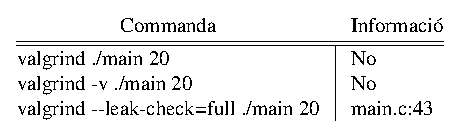
\includegraphics{1Entrega/tblAbre.eps}
\end{figure}

On la línia 43 és:

\begin{lstlisting}[language=C]
  /* Allocate memory for tree */
  tree = (RBTree *) malloc(sizeof(RBTree));
\end{lstlisting}

Ara, per a solucionar-ho, editarem la funció:
\begin{lstlisting}[language=C]
  /* Delete the tree */
  deleteTree(tree);
\end{lstlisting}

Problema resolt.


Ara tenim un problema, l'enunciat diu que només hem de fer cas als que tenen una llargada de 3!
Llavors això implicarà que sempre ens tocarà fer un free.
